\documentclass{acm}

% Pseudocode
\usepackage{amsmath}
\usepackage{algorithm}
\usepackage[noend]{algpseudocode}

\usepackage[justification=centering, labelfont=bf]{caption}

% Spacing between paragraphs
\newcommand{\subparagraph}{}
\usepackage{titlesec}
\titlespacing*{\section}{0pt}{1em}{1em}
\titlespacing*{\subsection}{0pt}{1em}{1em}
\titlespacing*{\subsubsection}{0pt}{1em}{1em}

\title{Log-Structured Merge Tree}
\subtitle{CS 265 Final Project, Spring '17}
\author{Jack Dent\\\email{jdent@college.harvard.edu}}

\begin{document}

\maketitle

\begin{abstract}
This work presents the design of a Log-Structured Merge Tree (LSM Tree), which serves as a standalone key-value store, as well as an implementation in C++. Various parameters give users given fine grained control over the tradeoff between the store's read and write throughput, and a number of optimisation as well as query parallelisation allow the store to increase the saturation of available hardware to optimise performance. Experimental results show that the store is able to achieve a write throughput of up to 300K and a read throughput of 30K on the test infrastructure.
\end{abstract}

\section{Introduction}

The LSM Tree has seen increasing adoption as an industry standard for modern key-value stores, both as standalone products and as components in larger database management systems (DBMSs). Facebook's RocksDB, Google's LevelDB, and Amazon's Dynamo are prominent examples of standalone key value stores that depend on LSM Trees as their primary storage layer. SQLite4, meanwhile, dropped the B-tree in favour of the LSM Tree as the main table store. By avoiding in-place updates and instead buffering all writes in main-memory, the LSM Tree vastly improves write throughput by amortising costly roundtrips to and from secondary storage over very many write operations. When the main-memory buffer becomes full, the LSM Tree flushes its entire contents to secondary storage. On disk, the LSM Tree stores a number of levels, each of which contain a number of ``runs'' whose size increases in proportion to the level depth. To increase the performance of point and range queries, the LSM Tree stores a number of auxiliary data structures in main-memory for each run. Bloom filters allow point queries to avoid searching runs that are known to not contain the search key. Fence pointers, meanwhile, establish bounds on the the subranges in run pages, allowing point and range queries to avoid having to read inconsequential pages into main-memory.

This paper presents the design and implementation of a parallelised LSM Tree that allows application users to control the tradeoff between read and write throughput by tuning the following parameters during initialization:

\pagebreak

\begin{enumerate}
\item \textbf{Buffer size, $b$:} controls the number of pages in the main-memory buffer, and therefore also affects the size of runs on secondary storage. Defaults to 1000, which gives the buffer a size of 4MB.
\item \textbf{Level fanout, $f$:} controls the size ratio between the levels. All levels can contain a maximum of $f$ runs, where the maximum size of the run increases exponentially in $f$. For example, the first level contains runs of size $bf$, the second level $bf^2$, and so forth. As will be discussed, the level fanout controls the tradeoff between read and write throughput. Defaults to 10.
\item \textbf{Tree depth, $d$:} controls the number of levels on disk, and as such the overall storage capacity of the tree. Defaults to 5.
\item \textbf{Thread count, $t$:} controls the number of worker threads dispatched to process queries in parallel. Defaults to 4.
\item \textbf{Bloom filter bits per entry, $r$:} controls the number of bits each entry receives in the bloom filter. Defaults to 0.5, which means that the bloom filter is two orders of magnitude smaller than the array of entries.
\end{enumerate}

\section{Design}

The LSM Tree has two primary components: an in-memory buffer, and a number of ``levels'' on secondary storage of progressively increasing size. For the purposes of this paper, a ``key/value entry'' is an compact C \texttt{struct} that contains two 4-byte integers, a key and a value, and whose total size is therefore $e=8$ bytes.

\subsection{Buffer design}

The ``buffer'' is an in-memory \texttt{std::set} of entry \texttt{structs}. The parameter $b$ controls the number of pages in the buffer, and the number of entries is thus given by $bp/e$, where $p$ is the size of a single page in bytes. Storing a buffer as a unsorted log would ensure optimal $O(1)$ write performance, but would require $O(bp/e)$ operations for point queries. On the other hand, storing the buffer as a sorted array would improve the performance of point queries to $O(\log(bp/e)$, but every insertion would cost $O(bp/e)$.

To balance the performance of reads and writes I used the \texttt{std::set} data structure, which implements a binary search tree and demonstrated a time complexity of $\Theta(\log(bp/e))$ for both lookup and insertion. Under most circumstances, the buffer will not be the bottleneck for workload throughput since the cost of secondary storage I/O will dominate query latencies. Under workloads that exhibit highly skewed query distributions or strong time contiguity within wider distrbutions, the buffer will again become important since the majority of queries will never make it to disk, and in this case a skip list will be most appropriate. Rather than attempting to optimise the buffer data structure, this project chose to focus on optimisations that applied across a broader range of workload distributions.

\subsection{Level design}

LSM Tree implementations can be divided into two categories based on their choice of merge policy. The first merge policy, known as \textit{leveling}, stores entire levels as single files that contain sorted key/value entries on disk. Leveled LSM Trees require a merge/sort between the buffer and first disk level every time the buffer becomes full, and also requires that entire levels are merge/sorted when upper levels become full. Since level size increases with depth, merging two levels that potentially contain millions of entries can take a significant amount of time unless the fanout $f$ is low, during which all queries to the tree are blocked. Thus, leveled LSM Trees are primarily optimised for high lookup throughput, rather than high update throughput. On the other hand, a \textit{tiered} LSM Tree makes updates less costly at the expense of reads. A tiered LSM Tree splits levels into multiple runs, and therefore avoids having to merge levels every time the buffer becomes full. Lookup queries become more expensive, however, since levels are no longer sorted, only the runs. As $f \rightarrow \infty$, a leveled LSM Tree becomes a sorted array and a tiered LSM Tree becomes a log.

\subsubsection{Runs}

I opted to build a write-optimised LSM Tree, and therefore decided to implement the tiering merge policy. In my design, a ``level'' holds a time-ordered collection of ``runs'' stored in a \texttt{std::deque}. A ``run'' is an in-memory data structure that holds a pointer to a file stored on disk, a fixed-size bloom filter, and fence pointers. The file stores a number of entries in ascending order, sorted by key. In the case of a crash, the store can recreate the bloom filter and the fence pointers for all runs from the entries on disk, although any entries in the buffer that have not been checkpointed will be lost. Every level contains a maximum of $f$ runs at any one time, and the maximum size of each run at level $l$ (in pages) is bounded by $O(bf^l)$. A run is not guaranteed to contain the maximum number of entries since the merge procedure removes duplicates, but runs in the same level will all have approximately the same size. The store never updates existing runs in place.

\subsubsection{Run ordering}

The store induces a global time-ordering across all runs, which fixes a pseudo-logical timestamp for each run. The global ordering is given first by level depth, and then by the position of the run within that level, where the most recent runs are stored at the front of the level \texttt{deque}. A single run will never contain more than one entry for a given key; on the other hand, there is no guarantee that different runs will not contain conflicting entries. The global ordering helps to ensure that the LSM Tree always gives preference to the most recent key/value pairing when searching and merging levels.

\subsubsection{Bloom filters}

Bloom filters improve the performance of point queries by reducing the number of secondary storage I/Os needed to search a run. When the store writes entries to a new run, it marks each entry as present in the bloom filter by hashing the key using three different functions and then setting the bit at each of the hashed positions to the value of 1 in a bitmask. For a given key, a bloom filter probe returns a negative result if any one of the three bits at the hashed positions of that key in the bitmask is 0. Since bloom filters allow false positives, the store will sometimes perform one unnecessary read I/O during GET queries in the case where the bloom filter incorrectly implies a relevant is present in the run on disk. Importantly, bloom filters never return false negatives, which implies that the store will never fail to discover an entry that actually exists within a disk level.

\subsubsection{Fence pointers}

Fence pointers improve the performance of point and range queries by providing information about the location of entries on disk, thus preventing the store from having to perform an expensive binary seek over the entire file. Each run stores fence pointers as a \texttt{std::vector} of keys, where the number of fence pointers is equal to the number of pages in the run, and the fence pointer at index $i$ contains the value of the first key in page $i$ of the run. Each run also stores an additional fence pointer that contains the maximum key over all its entries, which establishes an upper bound on the key range of the last page.

\begin{figure}
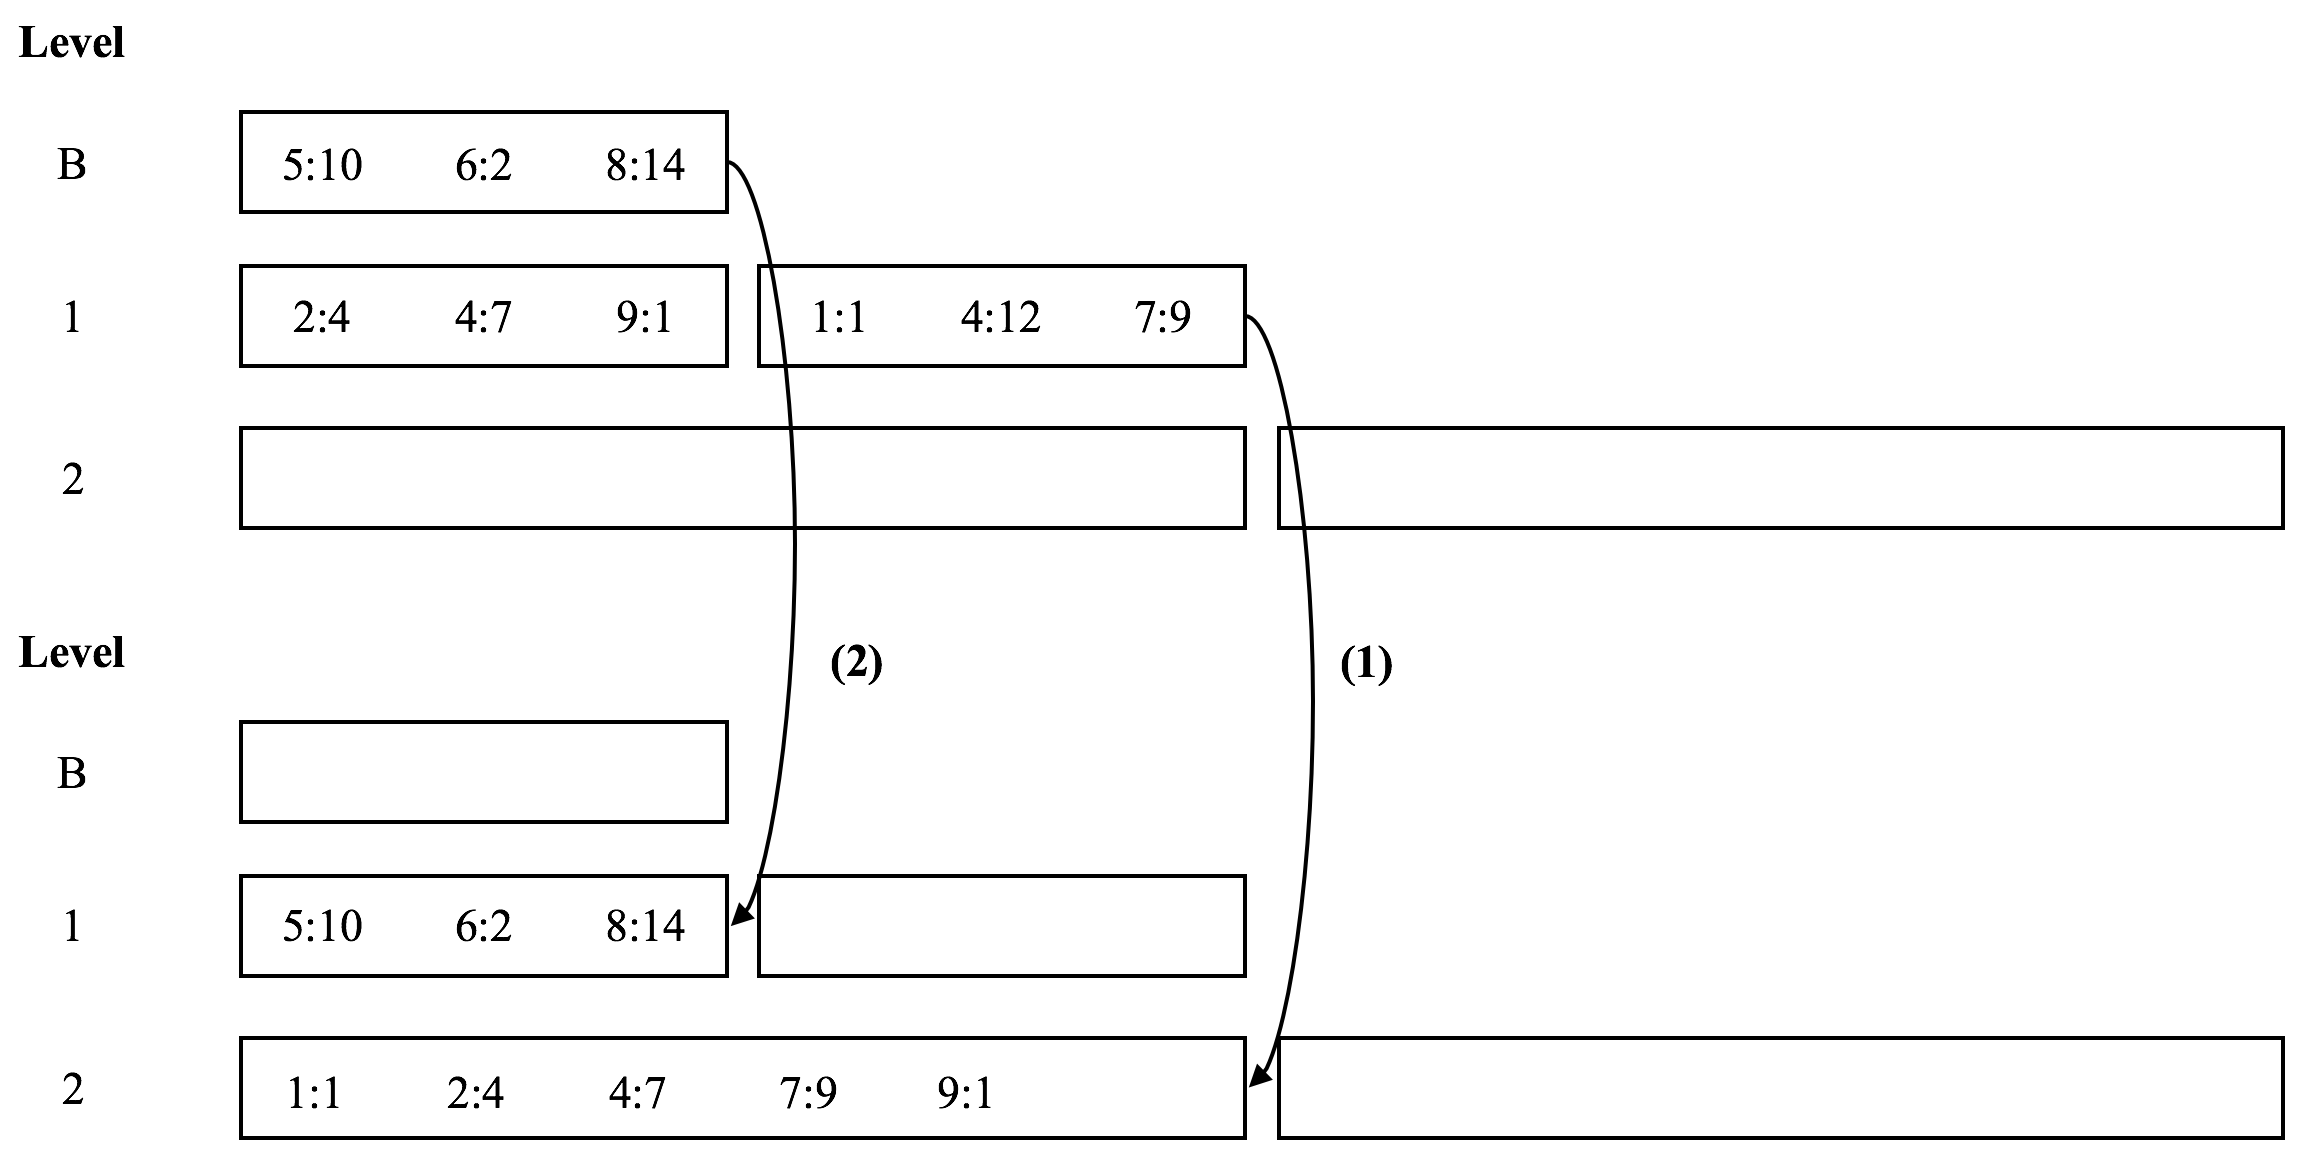
\includegraphics[width=3.33in]{merge}
\caption{The tiered merge policy for an LSM Tree with $f=2$, $d=3$, where the buffer contains exactly key/value entries. When the buffer (level B) becomes full, the LSM Tree must flush its entries to level 1 to make space for future PUT queries. However, since level 1 is full, the merge down procedure must first flush level 1 to level 2 (step 1). Since the first run in level 1 contains the entry 4:7 and the second contains 4:12, the \texttt{MergeSort} procedure ensures that only the more recent value, 4:7, is written to the third level. As such, the first run in the third level only contains 5 entries, although it has a capacity of $b \cdot f^{l-l} = 3 \times 2^1 = 6$. After completing step 1, the LSM Tree flushes the buffer to level 1, which is now empty.}
\label{fig:merge}
\end{figure}

\subsection{PUT queries}

The LSM Tree always inserts new key/value pairs into the buffer. If the buffer is full then the store will flush the buffer to disk before attempting to insert the key. If the first level is full, in that it contains exactly $f$ runs, the store will call \texttt{MergeDown(1)} before attempting to flush the buffer to the first level. When the \texttt{MergeDown} procedure terminates (if invoked), the LSM Tree creates a new run at the start of the first level, inserts every entry in the buffer setting the relevant bloom filter entries and fence pointers, and then empties the buffer. Thus, PUT queries always create at least one new run if the buffer is full.

\subsubsection{\texttt{MergeDown} policy}

The \texttt{MergeDown($l$)} procedure for clearing space in disk levels works as follows. First, if the current level $l$ already has capacity for a new run, the procedure terminates (line 4). If level $l+1$ does not have space for the entries in level $l$, it recursively calls \texttt{MergeDown($i+1$)} (lines 5-6). At line 7, it is guaranteed that level $l+1$ will contain at most $f-1$ runs, and also that a run in level $l+1$ has the capacity to store all $f$ runs in level $l$. The procedure then performs a merge/sort on all the runs in level $l$ (line 7) and writes the results to a new run at the start of level $l+1$ (line 8). The final stage of the procedure clears level $l$ of all runs and entries, since they will now be contained by level $l+1$.

\begin{algorithm}[b]
\caption{Merge down procedure}
\begin{algorithmic}[1]
\Procedure{MergeDown($l$)}{}
\State $n_l \gets \text{number of runs in level } l$
\State $n_{l+1} \gets \text{number of runs in level } l+1$
\If {$n_l < f$}
\Return
\EndIf
\If {$n_{l+1} = f$}
\State $\Call{MergeDown}{l+1}$
\EndIf
\State $r_{new} = \Call{MergeSort}{\text{runs in level } l}$
\State $\text{add } r_{new} \text{ to level } l + 1$
\State $\text{empty level } l$
\EndProcedure
\end{algorithmic}
\end{algorithm}

\subsubsection{\texttt{MergeSort}}

To merge $f$ runs, the LSM Tree invokes an $f$-way external \texttt{MergeSort} procedure. \texttt{MergeSort} is also responsible for both removing duplicate keys and pruning deleted entries from the final level. \texttt{MergeSort} pushes the first entry in each of the levels and the file pointer associated with that disk level onto a priority queue. The queue contains tuples of the form $(entry, timestamp, file)$ ordered first by the entry key and second by timestamp, which ensures that the store resolves key collisions in the correct order. While the priority queue is not empty, the procedure pops the first tuple and writes the entry to the new run if two conditions hold:

\begin{itemize}
  \item The current key is different to the last. If the current entry contains the same key as the previously seen entry, it is discarded to prevent duplicates. Since the priority queue gives precedence to runs with smaller logical timestamps in the case of key conflicts, \texttt{MergeSort} will always write the more recent entry to the new run.duplication.
  \item It is not the case that the new run is in the final level and the current entry is marked as deleted. Thus, we eventually remove deleted entries from the tree.
\end{itemize}

The \texttt{MergeSort} procedure makes sure both to set the entry's bits in the bloom filter, and to update the fence pointers in the new run whenever it writes an entry to disk. After writing an entry to disk, \texttt{MergeSort} checks to see if the file stream has been exhausted. If the file has remaining entries, the procedure pushes the new $(entry', timestamp, file)$ tuple back onto the priority queue, repeating this entire procedure until the queue is empty.

\subsubsection{Complexity}

A lower value of $f$ enforces a stricter global ordering over the entries and thus improves read performance at the expense of higher amortized writes costs. On the other hand, a higher value of $f$ reduces the frequency of the merge operation and therefore improves write throughput while penalising reads. The worst-case workload for updates occurs when all inserted keys are eliminated, which implies that all runs will have maximum capacity at all levels. Since there are at most $d$ levels in the tree, and since each key/value entry is merged at most once per level, entries are subject to at most $O(d)$ merge/sort operations. The write I/O cost of merging a single entry is $1/b$, and the amortized worst case I/O write complexity of the update procedure is therefore $O(\frac{d}{b})$. The \texttt{MergeDown} algorithm reads exactly as many pages as it writes in the worst case run of update operation, and assuming that the ratio of read I/O cost to write I/O cost is $\mu$, the total amortized I/O cost is therefore $O(\frac{d}{b} + \mu \cdot \frac{d}{b}) = O((1 + \mu) \cdot \frac{d}{b})$. After $n$ writes, the tree has depth at most $\log_f(n/b)$, which implies the update complexity is $O(\frac{1}{b} \cdot (1 + \mu) \cdot \log_f(n/b))$. Thus, the update cost decreases as $f$ increases, and when $f=n/b$, the insertion cost becomes $1/b \cdot (1 + \mu)$, which turns the store into a log.

\subsubsection{Parallelisation}

A typical value for the level fanout $f$ parameter used by many commercial LSM Trees (including LevelDB) is 10. With this setting, each level will contain at most 10 runs, and the merge procedure will always flush 10 runs to the next level when the current level reaches its capacity. Since this work used a machine with 4 cores, the multi-threaded \texttt{MergeSort} procedure did not exhibit a significant advantage over a single threaded approach.

Although this project did not experiment with larger values of $f$, the following procedure could improve the performance of PUT queries through parallelisation in those circumstances. When $f < c$, where $c$ is a tunable parameter, the LSM Tree should fall back to merging the entries in a single thread. Otherwise, the LSM Tree should uniformly partition the runs into subranges, and each thread should merge exactly one subrange, buffering the resulting array in main-memory. The main thread should wait for all of the threads to finish their merge procedures and then perform a $t$-way merge/sort over the buffers, writing the result to a new run in the appropriate level. As an alternative, a number of (potentially preemptable) background daemon threads could proactively merge together runs in levels with low capacity.

\subsection{GET queries}

The single-threaded store answers point queries by first searching the buffer, and then only searching the lower levels if no relevant entry was found. Searching the buffer does not perform an I/O operations and therefore has negligible cost unless the workload is heavily skewed, as discussed above (see ``Buffer design'' section). To search the lower levels, the LSM Tree searches every run in every level according to the global time-ordering.

To search for a key in a single run, the store first checks that the key is present in the bloom filter, and also that it falls within the fence pointer range. If either probe returns a negative, it is certain that the run file does not contain an entry for the specified key and the search can continue in the next run. Otherwise, the procedure performs a binary search over the fence pointer \texttt{vector} to find the index of the page it should read from secondary storage. By specifying a unique page for a given key within each run, the fence pointers thus allow the search procedure to avoid performing a logarithmic number of read I/Os to identify the relevant page. Finally, the procedure reads a single page into a buffer and attempts to find an entry for the specified key, continuing to the next run if no such entry could be found. If the procedure moves past the final run without finding a key, it concludes that no relevant entry exists. 

\subsubsection{Complexity}

To model the cost of GET queries, we first note that querying a missing key will require a full search over every level of the tree and that as such, worst case performance will be fairly common under many workloads. Thus, we model the complexity of GET queries by assuming a probe to every run.

Searching a run for a key takes at most one read I/O cost due to the fence pointers, and since each level contains $f$ runs, the total I/O cost of searching run $l$ is $O(f)$. However, the store only performs an unnecessary read I/O if the bloom fitler probe returns a false positive, since it stops the search as soon as it finds a run that run actually contains the entry. If we assume a constant false positive rate $\phi$ across all bloom filters, which can be tuned by the bits per entry parameter $r$, we only perform $O(\phi \cdot f)$ unnecessary read I/Os per level in the worst case. As such, the worst case I/O cost of searching all levels is $O\left(\phi \cdot f \cdot d\right)$. After $n$ writes, the tree has depth at most $\log_f(n/b)$, which implies the lookup complexity is $O(\phi \cdot f \cdot \log_f(n/b))$. Thus, the lookup cost increases as $f$ increases, and when $f=n/b$, the lookup cost becomes $O(\phi \cdot n/b)$.

\subsubsection{Parallelisation}

To parallelise GET queries, the store uses $t$ threads to search $t$ runs simultaneously. Each thread has access to the four variables in shared memory: a spinlock to enforce mutual exclusion, a run counter that is initially set to 0, a integer id that is initially set to -1, and a value variable. Threads execute the following loop to search runs.

First, the thread stores the current value of the counter in a private variable, and then atomically increments the value of the shared counter using the spinlock. If the integer id is still -1, or if the private counter variable is greater than the total number of runs over the entire tree, the thread ends its search loop. Otherwise, the thread searches the run whose timestamp is equal to the private counter variable by following the procedure outlined in the single threaded approach. If no entry was found in the run, the thread executes the next iteration of the loop. On the other hand, if the run probe discovered an entry, the thread acquires the spinlock and updates the shared value and integer id variables to the discovered entry's value and the private counter respectively. The main thread waits for all threads to end their loops.

Intuitively, threads keep searching for entries until another thread has discovered a relevant entry, or until they have either exhausted the tree. The shared integer id is used to ensure that the entries in more recent runs are always given precedence than those further down the tree. Barring thread management overhead, the speed of GET queries should increase in proportion to the number of threads up to the optimal value for the hardware.

\subsection{DELETE queries}

DELETE queries are handled almost identically to PUT queries. To delete a key, the LSM Tree inserts the key with a tombstone value. By restricting the range of possible values to $[-2147483647, 2147483647]$, it is possible to assign $-2147483648$, the minimum value of a 32 bit integer, as the tombstone. Alternatively, if we did not want to restrict the value range, we could instead increase the size of the entries stored by the tree by an additional byte, which would indicate whether the deletion status of the associated key. Another option would be to store a deletion list in each run.

We keep tombstone entries until they reach the final level. When an entry reaches the final level, it is guaranteed that there are no deeper levels containing outdated values for that key which allows the store to remove tombstone entries, thereby preventing the tree from becoming saturated with deleted key/value pairings.

\subsection{RANGE queries}

The single-threaded store searches for subranges in the buffer and each run independently, buffers the results into main-memory vectors, and then merge/sorts the subrange vectors according to the global time ordering.

To search for a subrange in the buffer, the store performs a binary search to find the lower and upper bounds, copies the results into a new \texttt{vector}, and pushes that \texttt{vector} onto a queue.

The procedure then loops over the runs in order, building a subrange \texttt{vector} for each. To search for a subrange in a single run, the store performs two binary searches over the fence pointers to find the indices of the start and end pages for the given subrange, and then reads the contiguous set of pages between these indices into main memory. The store then filters the array of entries to the specified subrange and pushes the resulting vector onto a queue.

\subsubsection{Complexity}

The cost of RANGE queries depends entirely on the parameter values for the start and end keys. For example when the start key is minimised and the end key is maximised, the store will have to perform a read I/O for every single page in the tree to collect all the values.

Assuming that the start key is $k_s$ and the end key is $k_s + \Delta$, the range can span at most $ \frac{e \cdot \Delta}{p}$, and the store will thus read at most $O(\frac{e \cdot \Delta}{p})$ pages to find the subrange for a given run. The total I/O cost of searching a level is therefore $O(f \cdot \frac{e \cdot \Delta}{p})$. It follows that the complexity of RANGE queries is $O(d \cdot f \cdot \frac{e \cdot \Delta}{p})$. When $\Delta < p$, the page size, the complexity equals that of a point query scaled by a factor of $\phi$, since the only difference between the queries is in the use of bloom filters.

\subsubsection{Parallelisation}

To parallelise RANGE queries, the store uses $t$ threads to find subranges in $t$ runs simultaneously. Each thread has access to the three variables in shared memory: a spinlock to enforce mutual exclusion, an atomic counter that is initially set to 0, and a C++ \texttt{map} that associats run timestamps with subranges. Threads execute the following loop to search runs.

First, the thread stores the current value of the counter in a private variable, and then atomically increments the value of the shared counter. If the private counter variable is greater than the total number of runs over the entire tree, the thread ends its search loop. Otherwise, the thread finds the subrange in the run whose timestamp is equal to the private counter variable by following the procedure outlined in the single threaded approach. Finally, the thread acquires the spinlock and associates the discovered subrange with the private counter variable in the map. 

The main thread waits for all threads to end their loops and then merge/sorts the in-memory subrange buffers, giving precedence to subranges with lower ids when resolving merge conflicts. Barring thread management overhead, the speed of GET queries should increase in proportion to the number of threads up to the optimal value for the hardware.

\subsection{LOAD queries}

LOAD queries stream a binary file of key/value pairs, inserting each into the store in the sequence they occur. Thus, a LOAD query is almost identical to a series of independent PUT queries, with the one exception that it parses binary rather than ASCII data.

\section{Optimisations}

\subsection{Thread pool}

A ``thread pool'', a reusable pool of kernel threads, removes the overhead of creating a new set of threads after each query. The number of threads in the threadpool should be tuned to optimal value for the hardware, which will often be proportional the number of cores on the machine. The implementation used a condition variable to wake up kernel threads when new work is pushed onto the queue. For high saturation workloads, an alternative thread pool implementation could make use of \texttt{thread::yield} instead to prevent threads from sleeping between queries, although in this case cores would always be at 100\% CPU utilisation.

\subsection{mmap}

In independent experiments, \texttt{mmap} proved to be faster than the C++ \texttt{ifstream} and \texttt{ofstream} file abstractions both for sequential and random access. I therefore implemented \texttt{mmap} for every read and write I/O operation. Since the fence pointers imply that all I/Os will be page aligned, \texttt{mmap} was also a natural match.

Additionally, \texttt{mmap} demonstrated exceptional performance when I experimented with reducing the fence pointer to page ratio to save space in main-memory. When fence pointers refer to a collection of pages rather than just a single page, the most efficient way to find a key inside a page range is to perform a binary search over the disk pages. \texttt{mmap} proved to be an order of magnitude faster for randomly accessing pages than issuing separate \texttt{lseek} system calls during the binary search.

\section{Experimental results}

All experiments were run on a machine with a 2.8 GHz Intel Core I7 processors 16 GB of 1600 MHZ DDR3 random access memory, and 500 GB of SSD secondary storage. All experiments were run with a minimum workload size of 10,000,000 queries, and the observed values for read and write througput were calculated from a workload size of 100,000,000 queries.

\subsection{Effect of workload distribution on throughput}

\begin{table}[t]
\centering
\begin{tabular}{c|c|c|}
\cline{2-3}
\multicolumn{1}{l|}{} & \multicolumn{2}{c|}{\textbf{Distribution}} \\ \cline{2-3} 
 & \textbf{Uniform} & \textbf{Gaussian} \\ \hline
\multicolumn{1}{|c|}{\textbf{Read throughput}} & 28K & 43K \\ \hline
\multicolumn{1}{|c|}{\textbf{Write throughput}} & 305K & 314K \\ \hline
\end{tabular}
\caption{Read and write for an LSM Tree with $b = 1000$, $t = 4$, and $f = 10$.}
\vspace{-2em}
\end{table}

Over a uniform workload of 100,000,000 queries with $b = 1000$, $t = 4$, and $f = 10$, the store demonstrated a write throughput of 305,000 entries per second for PUT queries, and a read throughput of 28,000 entries per second for GET queries. For a workload with Gaussian distributions, the write throughput rose slightly. Since PUT queries overwrite existing keys in the buffer, the buffer is flushed less often under a Gaussian workload. Additionally, fewer entries need to be written to disk when merging runs, which improves the write performance. The read throughput rose by a factor of roughly 1.5X, since GET queries are more likely to find entries in earlier levels in the tree, thus preventing deeper searches.

Using an external skip list implementation, the write throughput doubled to approximately 600,000 entries per second, while the read throughput rose very slightly under Gaussian workloads. Further profiling confirmed that the buffer \texttt{std::set} implementation was a significant bottleneck on write performance for large values of $b$, since the \texttt{std::set} spends a lot of time rebalancing the search tree. When the buffer is small, the cost of write I/Os dominates the main-memory insertion costs. When $b=1000$, on the other hand, the buffer contains three orders of magnitude more entries than can be written in a single write I/O, and therefore becomes a bottleneck on throughput.

\begin{figure}
\centering
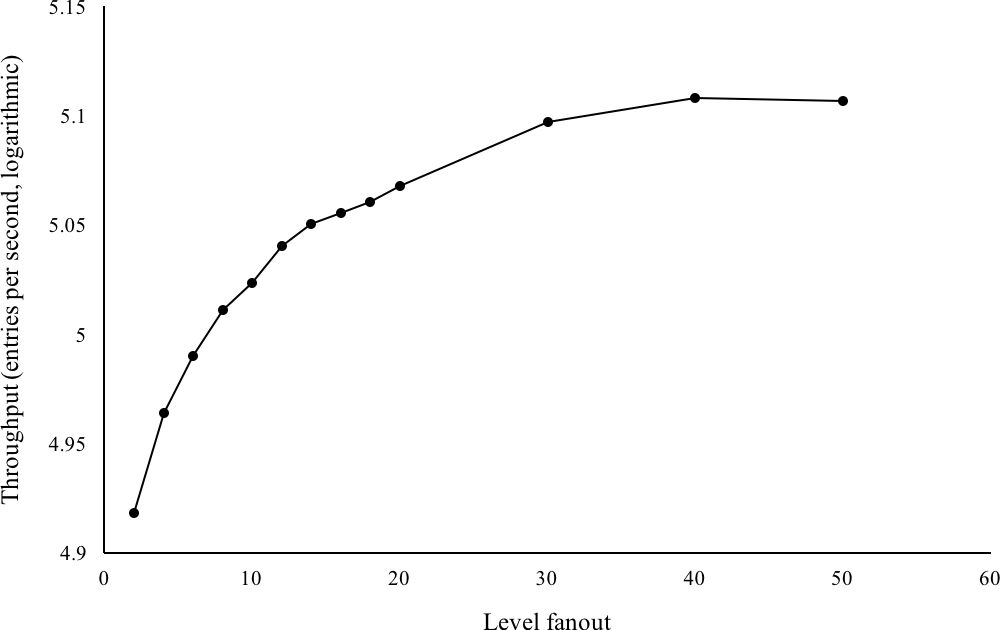
\includegraphics[width=3.33in]{fanout}
\caption{Effect of level fanout on PUT query throughput when $b=1$}
\end{figure}

\subsection{Effect of varying $f$}

Figure 2 shows the effect of varying the parameter $f$ over a uniform workload with $b = 1000$. As predicted by the models, increasing the level fanout causes an increase in write throughput up to a fanout of around $f=30$, at which point the write throughput levels off. A similar effect was evident across a wide range of buffer sizes.

\subsection{Effect of varying $r$}

Figure 3 shows the effect of varying the parameter $r$ over a uniform workload with $b = 100$ and $f = 1000$. Setting such a large fanout ensured that all entries were written to the first level, and thus isolated the effects of varying the bloom filter size. When $r=0.5$, the bloom filter size for each run is roughly 3KB since the runs in the first level all contain a maximum of 51,200 entries, which is two order magnitudes smaller than the file size. When $r=8$, the bloom filter size is approximately 50KB, which is only order of magnitude smaller than the file size.

As predicted by the models, increasing the bloom filter size increases the read throughput. Whereas the read throughput is only 10K entries per second when $r=0.5$ over a uniform workload with a cache miss ratio of 0.5, the throughput more than doubles to 25K when $r=8.0$.

\begin{figure}
\centering
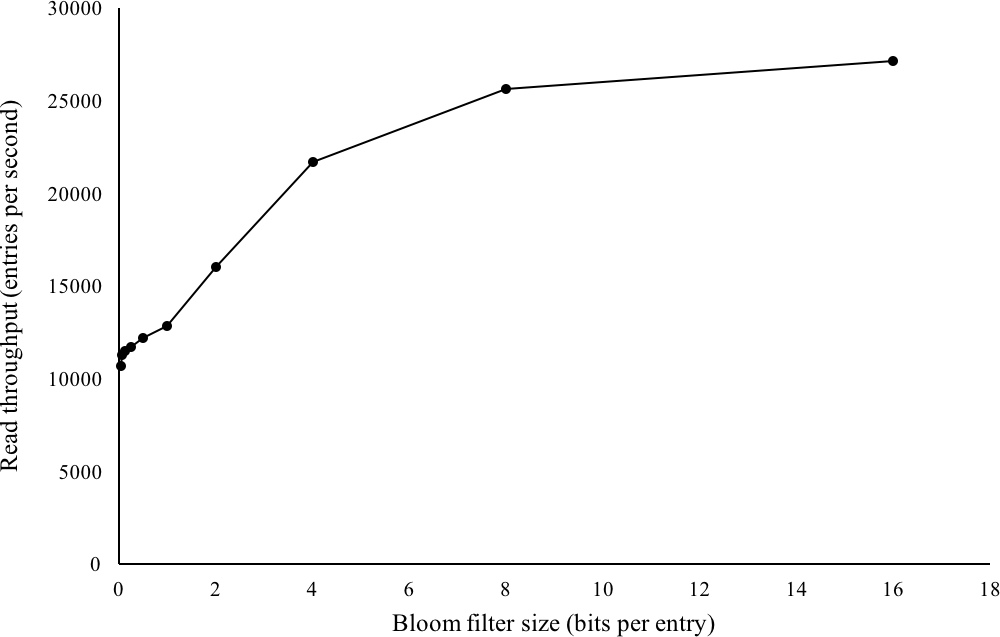
\includegraphics[width=3.33in]{bfratio}
\caption{Effect of bloom filte size on GET query throughput when $b=100$ and $f=1000$}
\end{figure}


\section{Conclusion and future work}

This paper presented the design for a Log-Structure Merge Tree, a standalone key-value store that has demonstrated high write throughput. The LSM Tree in this paper used a merging policy of \textit{tiering} to optimise the store for write throughput, but also gave users fine grained control over the tradeoff between read and write performance through various initializatoin parameters. The experimental section confirmed that users could vary the throughput characteristics of the tree by varying the level fanout parameter, $f$, and the bloom filter ratio parameter, $r$, according to the expected workload distribution.

The LSM Tree made a number of optimisations to improve both read and write throughput simultaneously, thereby shifting the entire throughput Pareto curve towards the origin. Parallelisation of GET and RANGE queries increased the throughput in proportion to the number of threads for both types of operation, up to the optimal thread limit for the given hardware. Likewise, using \texttt{mmap} rather than C++ file streams doubled the performance of both read and write I/O operations, which increased the throughput of GET, RANGE and PUT queries.

Future work should experiment with making further optimisations to the buffer data structure. The skip list implementation already demonstrated that the choice of main-memory data structure can have a significant affect on write throughput and with further optimisations, the LSM Tree shows great promise of achieving a throughput of up to one million entries per second for uniform workload distributions, and up to two million entries per second for skewed workload distributions.

Concurrency could further increase the performance of the both GET and PUT queries. Batching GET queries together could result in significant performance improvements for skewed workloads by combining and thus reducing the number of required secondary storage read I/Os. A background merge daemon could vastly increase the performance of PUT queries by proactively clearing space in the higher levels during GET and RANGE queries, such that fewer levels need to be merged during PUT queries. As a final optimisation, the C++ implementation should integrate the highly performant thread pool from Facebook's folly/wangle libraries to reduce parallelisation overhead.

\end{document}
